\documentclass[12pt]{article}
\usepackage[margin=25.4mm]{geometry}
\usepackage{graphicx}
\usepackage{hyperref}
\usepackage{amsmath}
\hypersetup{
   colorlinks=true,
   linkcolor=blue,
   filecolor=magenta,
   urlcolor=cyan,
}

\begin{document}
\title{
Setting up udev rules to identify USB devices on two TS-590SG transceivers
}
\author{
Kevin Schmidt, W9CF\\
6510 South Roosevelt Street\\
Tempe, Arizona 85283 USA\\
}
\date{}
\maketitle

\section{Introduction}
I began using SO2R with a Elecraft K2 and a Ten-Tec Corsair. Since then
I have upgraded each by buying used Kenwood TS-590SG rigs. Both of
these came with the SO-3 temperature compensated crystal oscillator
and the VGS-1 voice guide recorder/player/annunciator.
The only difference is cosmetic,
one of the rigs is an anniversary edition. They are otherwise identical.

Fortunately, the internal Silicon Labs CP210x USB serial adapters have
unique serial numbers. Unfortunately, the internal PCM2903B Audio codecs
do not. My shack computer dual boots linux and Windows 10, but I nearly
always use linux. These notes are how I set up udev to identify which
rig is which and give the serial and sound-card devices unique names.

\section{Internal serial Ports}
The serial ports have unique serial numbers. I added the udev rules
\begin{verbatim}
SUBSYSTEM=="tty", ATTRS{idVendor}=="10c4", ATTRS{idProduct}=="ea60",
ATTRS{serial}=="0567003D1908", SYMLINK+="ttyTS590sg_a", GROUP="dialout",
MODE="0660"

SUBSYSTEM=="tty", ATTRS{idVendor}=="10c4", ATTRS{idProduct}=="ea60",
ATTRS{serial}=="05670043DF58", SYMLINK+="ttyTS590sg_b", GROUP="dialout",
MODE="0660"
\end{verbatim}
to the file
\begin{verbatim}
/etc/udev/rules.d/90-serial-ports.rules
\end{verbatim}
{\em These udev rules each need to be on a single line with no line breaks!}

In addition to the USB Vendor and Product, I have included
the serial number. This is reported by turning on the power to the
TS-590SG and noting that the USB serial port device
\text{/dev/ttyUSB0} or \text{/dev/ttyUSB1} etc. appears, and then
doing an udevadm attribute walk to discover the serial number
\begin{verbatim}
udevadm info -a -n /dev/ttyUSB0
\end{verbatim}

With these rules, the serial devices
\text{/dev/ttyTS590sg\_a} and \text{/dev/ttyTS590sg\_b} are uniquely
associated with the correct rig.

\section{Internal USB sound Cards}
Unfortunately, there are no serial numbers associated with the TS590SG
internal sound devices. The most straightforward method to associate
stable unique names with each soundcard would be to always plug them
into the same USB ports, and this was my initial method. 


After including the serial rules above, I found
the KERNEL value to use in the KERNELS to match the internal hub in the radio.
I wrote the details as comments in the rules file.
Plugging into a different USB port on the computer would
require redoing this. To use this method, add the file
\begin{verbatim}
/etc/udev/rules.d/99-usb-audio.rules
\end{verbatim}
with contents:
\begin{verbatim}
#KERNELS is set to the KERNELS value for the internal TS590SG hub
#which corresponds to the physical USB port. The serial port serial
#number is used in 90-serial-ports.rules to alias the TS590SG serial
#ports to /dev/ttyTS590sg_a and /dev/ttyTS590sg_b. Therefore plugging
#in the TS590SG USB cable, powering it on, and using
#udevadm info -n /dev/ttyTS590sg_a -a
#or
#udevadm info -n /dev/ttyTS590sg_b -a
#will show the correct KERNELS value to use to get the corresponding
#audio device.
#Look for the parent device with idProduct 2512 and idVendor 0424.
#
ACTION=="change", SUBSYSTEM=="sound", KERNELS=="3-1.6.1", ATTR{id}="TS590SG_A",
ENV{PULSE_NAME}="TS590SG_A",ENV{ID_MODEL_FROM_DATABASE}="TS590SG_A"
ACTION=="change", SUBSYSTEM=="sound", KERNELS=="3-1.6.6", ATTR{id}="TS590SG_B",
ENV{PULSE_NAME}="TS590SG_B",ENV{ID_MODEL_FROM_DATABASE}="TS590SG_B"
\end{verbatim}

Looking at the udev rules for the sound cards, the default linux
sound card rules need to wait until all the sound card devices are detected
before completing. I therefore assumed that by the time that the
sound card change event occured, the serial port would be set up,
but see below for caveats.
I wrote a python script which given a 
TS-590SG sound card, walks up the usb device path until it finds the
TS-590SG internal hub. It then looks for a connected CP210x and
uses its serial number to identify the correct radio.

The following is my current configuration in 99-usb-audio.rules

\begin{verbatim}
#
# Here ts590sg.py walks walks up the DEVPATH environment variable until it
# finds the idProduct and idVendor of the internal hub of the TS590SG, it
# then walks down the subdirectories until it finds the idProduct and idVendor
# of the UART. It checks that serial number to tell which rig is which
#
ACTION=="change", SUBSYSTEM=="sound", ATTRS{idVendor}=="08bb",
ATTRS{idProduct}=="29b3", PROGRAM="/usr/local/udevprograms/ts590sg.py",
ATTR{id}="%c",ENV{PULSE_NAME}="%c",ENV{ID_MODEL_FROM_DATABASE}="%c"
\end{verbatim}

The python code returns either TS590SG\_A or TS590SG\_B which is substituted
for the pulse audio names and IDs. It is:

\begin{verbatim}
#!/usr/bin/env python3

#TS590SG internal hub ids
hubIdVendor = "0424"
hubIdProduct = "2512"
#TS590SG UARTs
UartIdVendor = "10c4"
UartIdProduct = "ea60"
UartSerialA = "0567003D1908"
UartSerialB = "05670043DF58"

import os
import sys
path = '/sys' + os.environ["DEVPATH"]
count = 0
vendor = ""
product = ""
#Walk up the devpath to find the TS590SG internal usb hub
while path != '/':
   if 'devpath' in os.listdir(path):
      count += 1
      if count == 2:
         with open(path + '/idVendor') as f:
            vendor = f.readline().rstrip()
         with open(path + '/idProduct') as f:
            product = f.readline().rstrip()
         break
   path = os.path.dirname(path)

#Do a sanity check that the ids are correct, then find the subdirectory
#for the UART. Read the Serial number to identify the rig.
if (vendor == hubIdVendor) and (product == hubIdProduct):
   subdirs = [f.path for f in os.scandir(path) if f.is_dir() and not f.is_symlink()]
   for d in subdirs:
      if 'devpath' in os.listdir(d):
         with open(d + '/idVendor') as f:
            vendor = f.readline().rstrip()
         with open(d + '/idProduct') as f:
            product = f.readline().rstrip()
         if (vendor == UartIdVendor) and (product == UartIdProduct):
            with open(d + '/serial') as f:
               serial = f.readline().rstrip()
               if serial == UartSerialA:
                  print("TS590SG_A")
                  sys.exit(0)
               elif serial == UartSerialB:
                  print("TS590SG_B")
                  sys.exit(0)

sys.exit(1)
\end{verbatim}

With this change, the pulse audio volume control shows the rig audio
devices with easy to identify names as shown in fig. \ref{f1}.
\begin{figure}
\begin{center}
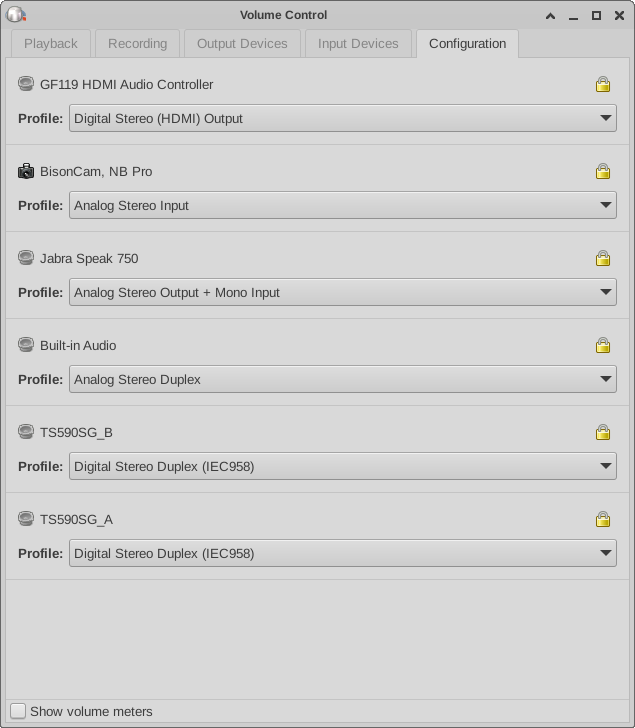
\includegraphics[width=.9\textwidth]{pulse_volume.png}
\end{center}
\caption{A screenshot of the pulse audio volume control showing the
sound card configuration with the easily identified
names TS590SG\_A and TS590SG\_B for the internal sound cards.}
\label{f1}
\end{figure}

Note! Looking at lsusb and the device number, the serial port has a
higher device number than the sound card device when DC is applied
to the TS590SG. This suggests that there could be a race condition
between the sound card udev rule getting triggered and the USB serial
port getting set up. I have not seen this problem. From the output
of udevadm monitor, it looks like the udev sound card processing in
/lib/udev/rules.d/78-sound-card.rules which waits for the card* device
to be setup takes enough time that the serial port is connected before
the change event occurs, which seems to be the last thing that happens
from the monitor output.  A failure to find the serial port should simply
cause the python code to exit with status 1, which will make the rule
not match, and the default names would be used for the sound card.

If there ever is a problem, I can revert to the previous method that
identifies the KERNELS value to use.

\end{document}
